\documentclass[10pt,handout]{beamer}
%\documentclass[10pt]{beamer}
\usepackage[english]{babel} % Anpassa efter svenska. Ger svensk logga.
\usepackage[utf8]{inputenc} % Anpassa efter linux
\usepackage{graphicx}
\usetheme{Uppsala}
%\usecolortheme{UU} % Anpassa efter UU:s frger och logga
%\hypersetup{pdfpagemode=FullScreen} % Adobe Reader ska ppna fullskrm
\setbeamertemplate{itemize items}[circle]

% \usepackage{beamerthemesplit}
\usepackage{amsmath}
\usepackage{amssymb}
% \usepackage{graphics}
% \usepackage{graphicx}
% \usepackage{epsfig}
% \usepackage[latin1]{inputenc}
 \usepackage{color}
% \usepackage{fancybox}
% \usepackage{psfrag}
% \usepackage[english]{babel}

\usepackage{array}
\usepackage{multirow}

 \setbeamertemplate{footline}{\hfill\insertframenumber/\inserttotalframenumber}


%library(tinytex)
%tlmgr_install('csquotes')
\usepackage{csquotes}

%\usepackage{bm}
%\usepackage{natbib}
\newcommand{\bfm}[1]   {\mbox{\boldmath{${#1}$}}}
\newcommand{\Prob}   {\mbox{\textnormal{P}}}
\def\eqd{\,{\buildrel d \over =}\,}
\DeclareMathOperator{\E}{\mathbb{E}}


\newcommand\MyBox[2]{
  \fbox{\lower0.75cm
    \vbox to 1.7cm{\vfil
      \hbox to 1.7cm{\hfil\parbox{1.4cm}{#1\\#2}\hfil}
      \vfil}%
  }%
}

%%%%%%%%%%%%%%%%%%%%%%%%%%%%%%%%%%%%%%%%%%%%%%%%%%%%%%%%%%%%%%%%%%

\setlength{\parskip}{3mm}
\title[]{{\color{black}Machine learning, big data and artificial intelligence -- Block 2}}
\author[]{M{\aa}ns Magnusson\\Department of Statistics, Uppsala University}
\date{November 2020}


\begin{document}

\frame{\titlepage
% \thispagestyle{empty}
}

%%%%%%%%%%%%%%%%%%%%%%%%%%%%%%%%%%%%%%%%%%%%%%%%%%%%%%%%%%%%%%%%%%


\begin{frame}{This weeks lectures}
\begin{itemize}
\item Regularization
\item Model Selection and Assement
\item Cross-Validation
\item Evaluate classification models
\end{itemize}
\end{frame}


%%%%%%%%%%%%%%%%%%%%%%%%%%%%%%%%%%%%%%%%%%%%%%%%%%%%%%%%%%%%%%%%%%


\section{Model Predictive Performance}
\frame{\sectionpage}

\begin{frame}{Previous Model Evaluation}
In the past, we have used a large number of tools for assessing models, e.g.:

\begin{itemize}
\item Various plots
\item Residuals
\item Leverage, Cook's distance
\item p-values
\item $R^2$
\end{itemize}

That is, they only tell us {\color{uured}how well the model fits the data}, and diagnose the model. \pause

The focus is usually \emph{estimation} or \emph{attribution}.
\end{frame}


\begin{frame}{Predictive Performance}

% We are looking at predictive performance here

\begin{itemize}

\item We are interested in how our model work when predicting a new observation \\

\begin{displayquote}
The generalization performance of a learning method relates to its prediction capability on \emph{independent} test data.

(Hastie et al, 2017, p. 219)
\end{displayquote}

\pause

\item Models can be overly optimistic -- the model can have a good fit but be poor at making predictions for new data\footnote{See e.g. Picard, R.R., Cook, R.D. (1984). Cross-validation of regression models. \emph{Journal of the American Statistical Association}, \textbf{79(387)}, 575--583.}, a phenomenon known as {\color{uured}overfitting}.\\[3mm]

\end{itemize}

\end{frame}

\subsection{Measuring Performance}

\begin{frame}{Loss Functions (again)}

% We are looking at predictive performance here


\begin{itemize}

\item To assess the performance we use the loss function for a new unseen observation $y_0$, and the prediction of that observation $\hat{y}$
\[
L(y_0,\hat{y}_0)
\]\pause
\item This is quite general and we choose based $L$ based on what we want the model performe well on.\pause
\item Examples:
\begin{itemize}
\item Regression problems:
\[
    L(y_0,\hat{y}_0) =
\begin{cases}
    |y_0 - \hat{y}_0|\\
    (y_0 - \hat{y}_0)^2
\end{cases}
\]\pause
\item Language models: Perplexity, Glue, Human annotation
\end{itemize}


\end{itemize}

\end{frame}


\begin{frame}{Confusion Matrix}


\noindent
%\centering
\renewcommand\arraystretch{1.5}
\setlength\tabcolsep{0pt}
\begin{tabular}{c >{\bfseries}r @{\hspace{0.7em}}c @{\hspace{0.4em}}c}
  \multirow{10}{*}{\parbox{1.1cm}{\bfseries\raggedleft Actual\\ Value}} &
    & \multicolumn{2}{c}{\bfseries Prediction Outcome} \\
  & & $p_{p}$ & $n_{p}$ \\
  & $p_{a}$ & \MyBox{True}{Positive} & \MyBox{False}{Negative} \\[2.4em]
  & $n_{a}$ & \MyBox{False}{Positive} & \MyBox{True}{Negative}
\end{tabular}


\end{frame}


\begin{frame}{Accuracy}

% We are looking at predictive performance here

\[
\text{Accuracy} = \frac{(\text{TP+TN})}{\text{(TP+FP+FN+TN)}}
\]\pause

What is the problem with Accuracy?
% Unbalanced samples

\end{frame}

\begin{frame}{Precision and Recall}


% Want to use when want to be sure about a prediction
\[
\text{Precision} = \frac{(\text{TP})}{\text{(TP+FP)}}
\]

Of the predicted positives, how many are actually positive?\pause

% Want to use when want to be sure about a prediction
\[
\text{Recall} = \text{Sensitivity} = \frac{(\text{TP})}{\text{(TP+FN)}}
\]

Of all positives, how many are predicted correctly?\pause

\[
\text{Specificity} = \frac{(\text{TN})}{\text{(TN+FP)}}
\]

Of all negative, how many are predicted correctly?\pause

% F1: Both good precision and recall
\[
\text{F1} = 2 \cdot \frac{(\text{Precision} \cdot \text{Recall})}{\text{(\text{Precision} + \text{Recall})}}
\]


\end{frame}


\begin{frame}{Example}

Say that we want to classify spam vs. ham. \\[3mm]\pause
%TODO: Images here

\begin{center}
\begin{tabular}{ l | c | c }
  & $\hat{y}=0$ & $\hat{y}=1$\\
  \hline
  $y=0$ & 515 & 91 \\
  $y=1$ & 85 & 569 \\
  \hline
\end{tabular}
\end{center}
The cell counts yield us estimates of
\begin{itemize}
\item Accuracy $P(\hat{y}=y)$: $\frac{515+569}{515+91+85+569}\approx 0.86$\\[3mm]\pause
\end{itemize}

In this example, we let $\hat{y}_i=1$ whenever $\hat{\pi}_i>0.5$. What if we choose another cut-off level $\hat{\pi}_i>\alpha$ instead?

\end{frame}


\begin{frame}{Classification tables}
Previous table, with acc. 86 \%, sens. 87 \% and spec. 85 \%:
\begin{center}
\begin{tabular}{ l | c | c }
 {\color{uured}$\alpha=0.5$} & $\hat{y}=0$ & $\hat{y}=1$\\
  \hline
  $y=0$ & 515 & 91 \\
  $y=1$ & 85 & 569 \\
  \hline
\end{tabular}
\end{center}
\pause
Now let $\alpha=0.3$ instead, so that we are more prone to say that $\hat{y}=1$:
\begin{center}
\begin{tabular}{ l | c | c }
  {\color{uured}$\alpha=0.3$} & $\hat{y}=0$ & $\hat{y}=1$\\
  \hline
  $y=0$ & 462 & 144 \\
  $y=1$ & 38 & 616 \\
  \hline
\end{tabular}
\end{center}
Accuracy: 86 \%, sensitivity: 94 \%, specificity: 76 \%.\\[3mm]
The sensitivity has increased, but the sensitivity has decreased...

\end{frame}



\begin{frame}{A more reasonable example}
Previous table, highly unbalanced. 1001 ham and 17 spam.

Our new classifier: Everything is ham!\pause

\begin{center}
\begin{tabular}{ l | c | c }
  & $\hat{y}=0$ & $\hat{y}=1$\\
  \hline
  $y=0$ & 1001 & 0 \\
  $y=1$ & 17 & 0 \\
  \hline
\end{tabular}
\end{center}
\pause

Accuracy: 98 \%! and sensitivity: 100 \%, specificity: 0 \%.\\[3mm]

\end{frame}


\begin{frame}{Cross-Entropy Loss}

\begin{itemize}
\item When we have probabilities $\hat{p}=\hat{y}_0$:
\[
L(y_0, \hat{p}) = - (y_0 \log{\hat{p}}) + ((1 - y_0) \log{(1- \hat{p})})
\]
Question: Do you recognize the loss function?
% Bernoulli negative log-likelihood?
\pause
\item Maximizing the likelihood is the same as minimizing the cross-entropy. \pause
\item Multi class generalization over $M$ classes
\[
L(\mathbf{y}_0, \hat{\mathbf{p}}) = - \sum^M_{j=1} y_{0,j} \log{\hat{p}_j}
\]
\end{itemize}

\end{frame}


\begin{frame}<handout:0>{Questions?}
Questions?
\end{frame}

%%%%%%%%%%%%%%%%%%%%%%%%%%%%%%%%%%%%%%%%%%%%%%%%%%%%%%%%%%%%%%%%%%


\section{Test error}
\frame{\sectionpage}

\begin{frame}{Test Error}

\begin{itemize}
\item The main error of interest - \emph{generalization error}
\item Conditional Test Error \\(Model performance for the \emph{training} data):
\[
\text{Err}_\mathcal{T} = \E_{Y,X}(L(Y,\hat{Y}(X) | \mathcal{T})
\]
\item Expected Test Error \\(Model performance over \emph{different} data):
\[
\text{Err} = \E_\mathcal{T}(\E_{Y,X}(L(Y,\hat{Y}(X)))
\]

\end{itemize}

\end{frame}


\subsection{Training Error}

\begin{frame}{Training Error}

\begin{itemize}
\item The Error the algorithm try to minimize
\item Error over the training sample:
\[
\overline{\text{err}} = \frac{1}{N} \sum_{i=1}^N L(y_i,\hat{y}_i)
\]
\item Can be seen as a Monte Carlo Appraximation over data

\end{itemize}

\end{frame}


\begin{frame}{How are training and test error related?}


\begin{figure}[h]
\caption{Test, training, and model complexity (Hastie et al, 2009, Figure 7)}
\centering
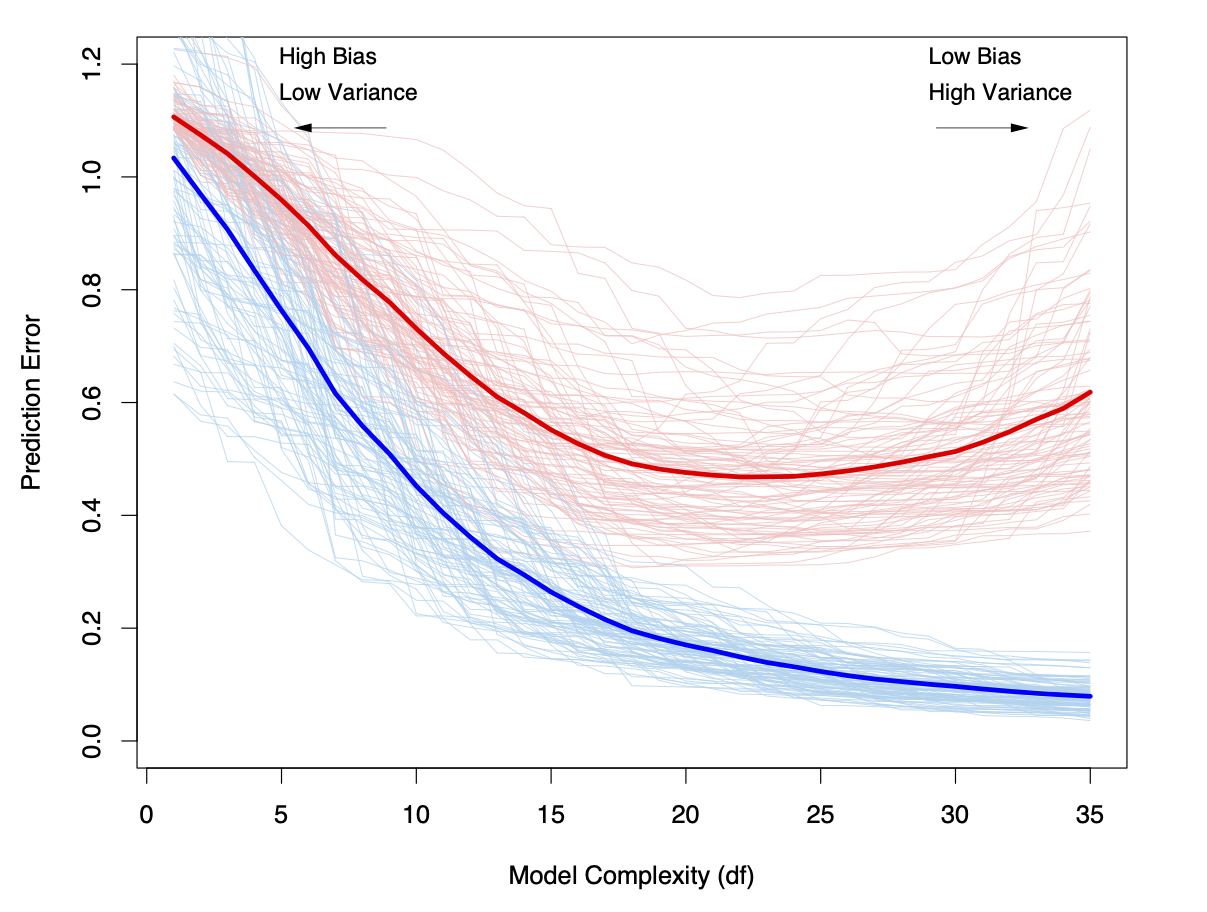
\includegraphics[width=0.8\textwidth]{figs/ESL_7_1.png}
\end{figure}

\end{frame}


\section{Model Assesment}

\begin{frame}{How to estimate the Test Error: Model Assesment}

\begin{itemize}
\item We set aside a \emph{test set} from the data
\item Use as the last step to \emph{estimate} the test error
\item Should only be used \emph{ONCE}\pause
\item Size of testset:
\begin{itemize}
\item Common suggestion 10\%
\item A statistical estimation problem
\end{itemize}
\end{itemize}

\end{frame}

\begin{frame}{Multiple Use of Test Set for Model Assesment}

\begin{itemize}
\item Say that we have $\hat{L}(\mathcal{T})$ an estimate of the loss on the test set given a training set
\item Lets say that we have $i \in \{1,...,M\}$ be models trained on $M$ independent training sets $\mathcal{T}_i$ but they all have the same underlying error $L^*$
\item Then we can assume that
\[
\hat{L}_i(\mathcal{T}_i) \sim N(L^*, \sigma)
\]
\item What happens if we use the test set to pick the model?
\end{itemize}

\end{frame}

\begin{frame}<handout:0>{Questions?}
Questions?
\end{frame}

%%%%%%%%%%%%%%%%%%%%%%%%%%%%%%%%%%%%%%%%%%%%%%%%%%%%%%%%%%%%%%%%%%


\section{Model Selection}
\frame{\sectionpage}


\begin{frame}{Model Selection}
\begin{itemize}
\item We want to select a model based on performance.
\item Important when using hyperparameters (as in regularization)
\end{itemize}

\end{frame}


\subsection{Bias and Variance}


\begin{frame}{Bias and Variance}

Assume we have the following data generating process:
\[
Y = f(X) + \epsilon\,,
\]
where $\E(\epsilon)=0$ and $V(\epsilon)=\sigma_\epsilon$.

\begin{align*}
\text{Err}(x_0) &= \E_{Y}\{(Y-\hat{f}(x_0))^2 | X = x_0\} \\
  &= \sigma^2_\epsilon + \{\E_Y(\hat{f}(x_0)) - f(x_0)\}^2 + \E\{\hat{f}(x_0) - \E_Y(\hat{f}(x_0))\}^2 \\
  &= \sigma^2_\epsilon + \text{Bias}^2(\hat{f}(x_0)) + V(\hat{f}(x_0))
\end{align*}

\begin{itemize}
\item \emph{Bias}: How close can we get to the true model
\item \emph{Variance}: The variability of the predictions
\item \emph{Irreducible error}: The best (theoretically) possible model
\end{itemize}

\end{frame}


\begin{frame}{Bias and Variance: Linear regression}

In linear regression we have:
\[
\hat{f}(x_i) = \hat{\beta} x_i
\]

This give us the following error decomposition:

\begin{align*}
\frac{1}{N}\sum^N_i \text{Err}(x_i) &= \sigma^2_\epsilon + \frac{1}{N}\sum^N_i (f(x_i) - E(\hat{f}(x_i))^2 + \frac{p}{N} \sigma^2_\epsilon
\end{align*}

\end{frame}


\begin{frame}{Bias and Variance}

\begin{figure}[h]
\caption{Test, training, and model complexity (Hastie et al, 2009, Figure 7)}
\centering
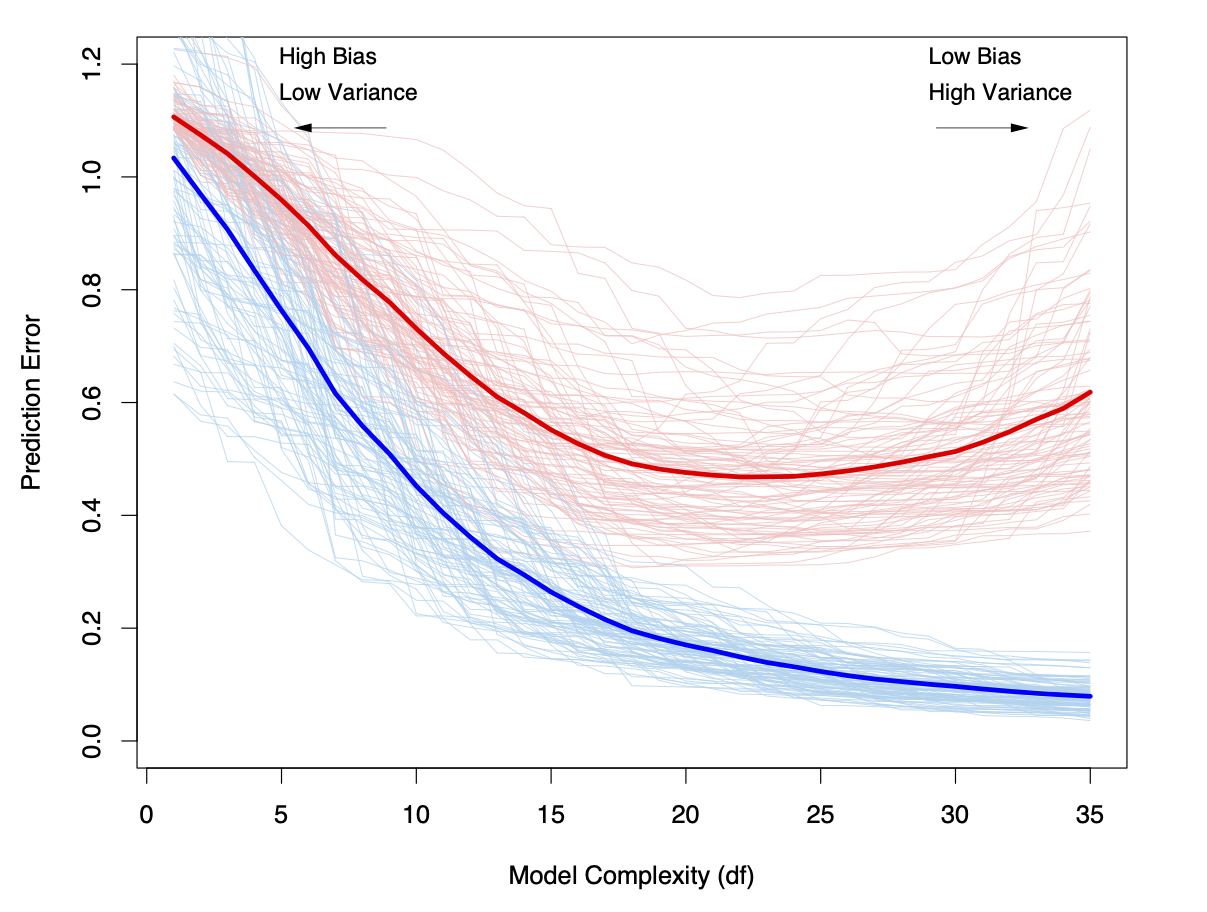
\includegraphics[width=0.65\textwidth]{figs/ESL_7_1.png}
\end{figure}

\begin{itemize}
\item High Bias: Underfit
\item High Variance: Overfit
\item High Irreducible error: No model is good
\end{itemize}

\end{frame}



\subsection{Optimism of Training Error}

\begin{frame}{Optimism of Training Error}

The in-sample test error:
\[
\text{Err}_\text{in} = \frac{1}{N}\sum^N_{i=1} \E_{Y^0}\{L(Y^0_i,\hat{f}(x_i))|\mathcal{T}\}\,,
\]
where $Y_{0,i}$ is a new response variable condition on $x_i$.\\[3mm]\pause

We have that
\[
\E_\mathbf{y} (\text{Err}_\text{in}) = \E_\mathbf{y}(\overline{\text{err}}) + \underbrace{\frac{2}{N}\sum^N_{i=1} \text{Cov}(\hat{y}_i,y_i)}_{\text{optimism}}\,,
\]
where $\overline{\text{err}}$ is the training error.

How could we create an optimistic classifier for the training data?

\end{frame}

\begin{frame}{Estimating Optimism}

\begin{itemize}
\item Under certain conditions we can estimate this optimism.
\item AIC, BIC etc are examples of this -- asymptotic predictive performance.
\end{itemize}



\end{frame}


\begin{frame}{Find the Optimism!}

\begin{figure}[h]
\caption{Test, training, and model complexity (Hastie et al, 2009, Figure 7)}
\centering
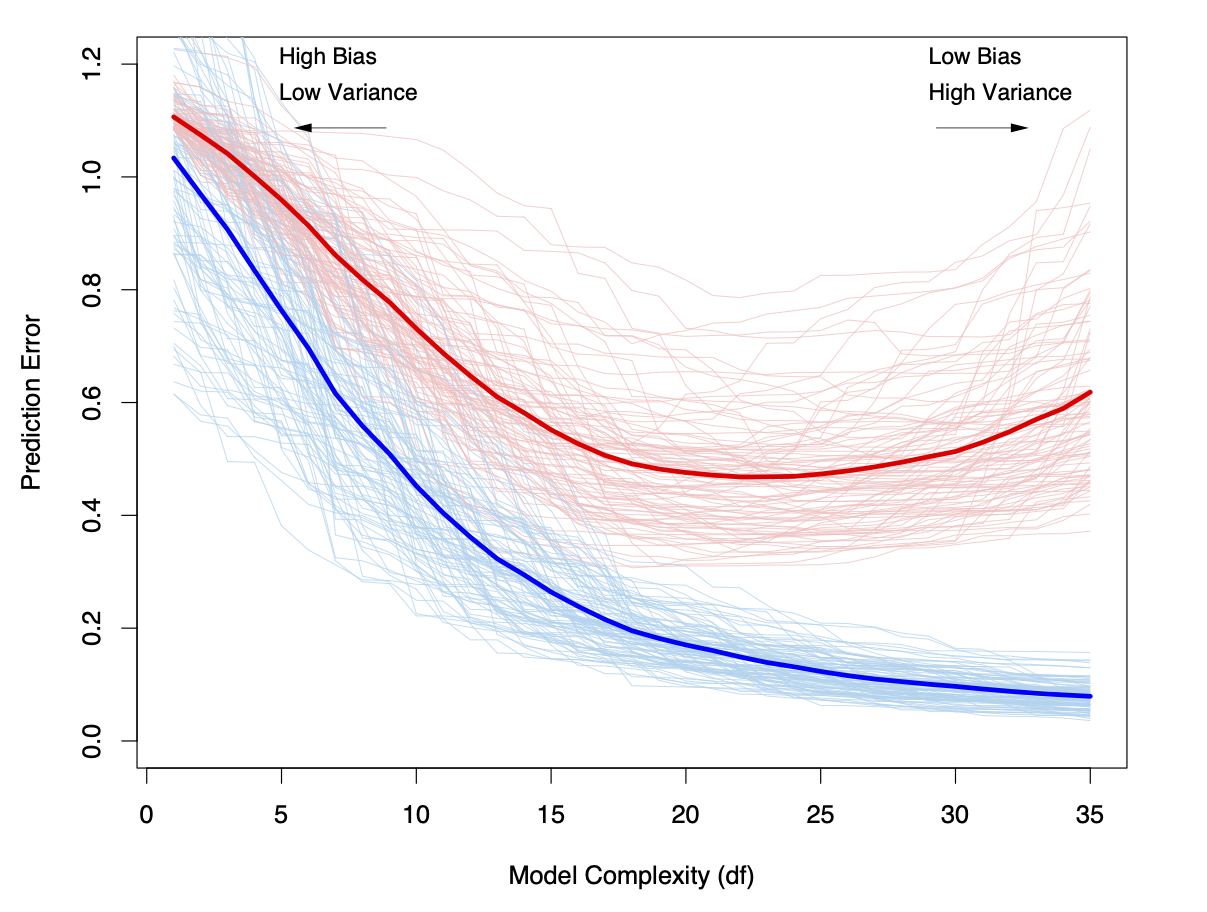
\includegraphics[width=0.8\textwidth]{figs/ESL_7_1.png}
\end{figure}

% Answer the diff between the red and blue line

\end{frame}



\begin{frame}<handout:0>{Questions?}
Questions?
\end{frame}

%%%%%%%%%%%%%%%%%%%%%%%%%%%%%%%%%%%%%%%%%%%%%%%%%%%%%%%%%%%%%%%%%%

\section{Cross-validation}
\frame{\sectionpage}


\begin{frame}{Cross-Valdidation}


We want to estimate $\text{Err}$ for different models and to choose the best model.\\[3mm]\pause

Cross-Validation is probably the most popular approach to estimate $\text{Err}$.

\begin{itemize}
\item The model is judged only on how well it does predictions for new data.\\[2mm]\pause
\item No need for rules-of-thumbs to verify that tests and estimators are applicable.\\[2mm]\pause
\item No need to worry about significance levels, standard errors etc.\\[2mm]\pause
\item Equally useful for frequentist, Bayesian and algorithmic methods (and these can easily be compared).\\[3mm]\pause
\end{itemize}


\end{frame}


\begin{frame}{Cross-Valdidation Algorithm}

\begin{figure}[h]
\caption{Cross-Validation (Hastie et al, 2009, p. 222, 242)}
\centering

\includegraphics[width=0.6\textwidth]{figs/ESL_test_train_val.png}
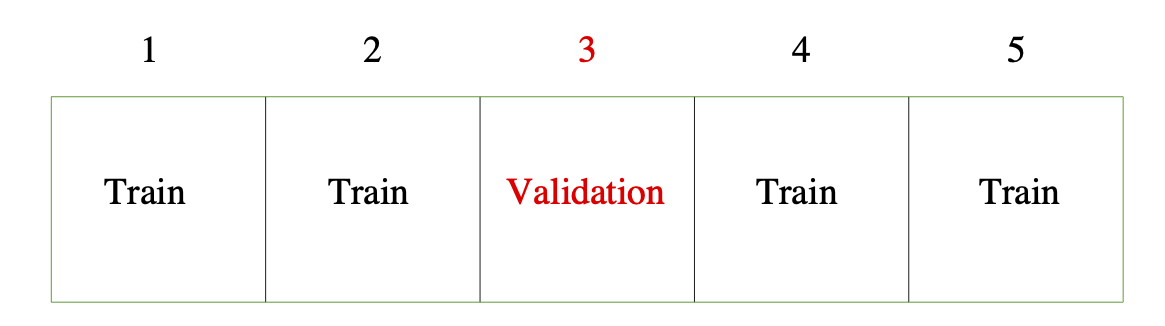
\includegraphics[width=0.6\textwidth]{figs/ESL_cross_val.png}
\end{figure}

\begin{enumerate}
\item Split data in $K$ folds
\item For each fold $k=1,2,...,K$
\begin{enumerate}
\item Use all samples except those in $k$ to build the predictive model
\item Use the model and predict the observations in fold $k$
\end{enumerate}
\end{enumerate}

\[
CV(\hat{f},\alpha) = \frac{1}{N}\sum^N_{i=1} L(y_i,\hat{y}_{-\kappa(i)}(x_i,\alpha)
\]

\end{frame}

\begin{frame}{The Bias of Cross-Valdidaton}

\begin{figure}[h]
\caption{Cross-Validation Bias (Hastie et al, 2009, Fig. 7.8)}
\centering
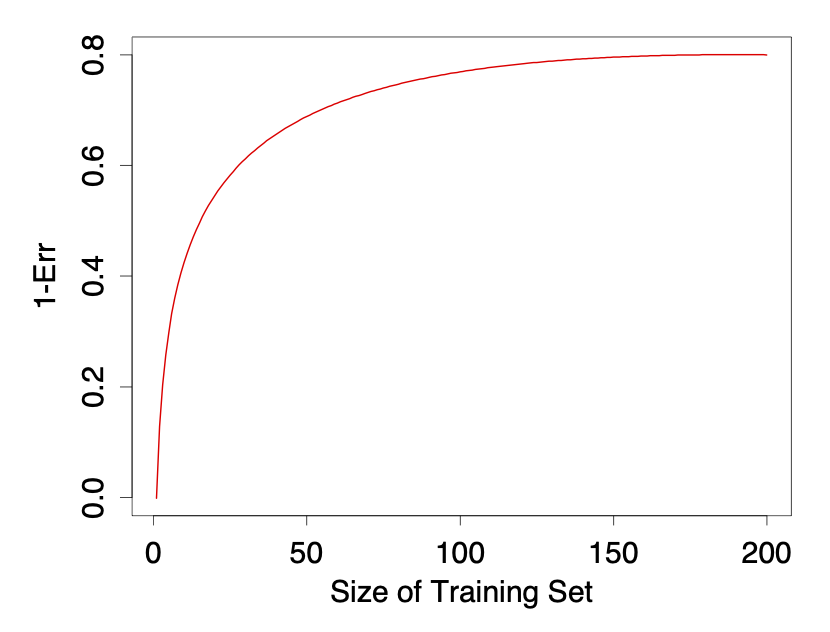
\includegraphics[width=0.9\textwidth]{figs/ESL_7_8.png}
\end{figure}

\end{frame}


\begin{frame}{Leave-One-Out Cross Validation}

\begin{itemize}
\item We set $K=N$
\item Benefits
\begin{itemize}
\item Almost unbiased estimate of $\text{Err}$
\item Can be less computationally costly is some situations
\end{itemize}
\item Drawbacks
\begin{itemize}
\item Higher Variance
\item Can be more computationally costly (naive implementation)
\end{itemize}
\end{itemize}

\end{frame}


\begin{frame}{Leave-One-Out Cross Validation}

\begin{figure}[h]
\caption{Cross-Validation Bias (Hastie et al, 2009, Fig. 7.14)}
\centering
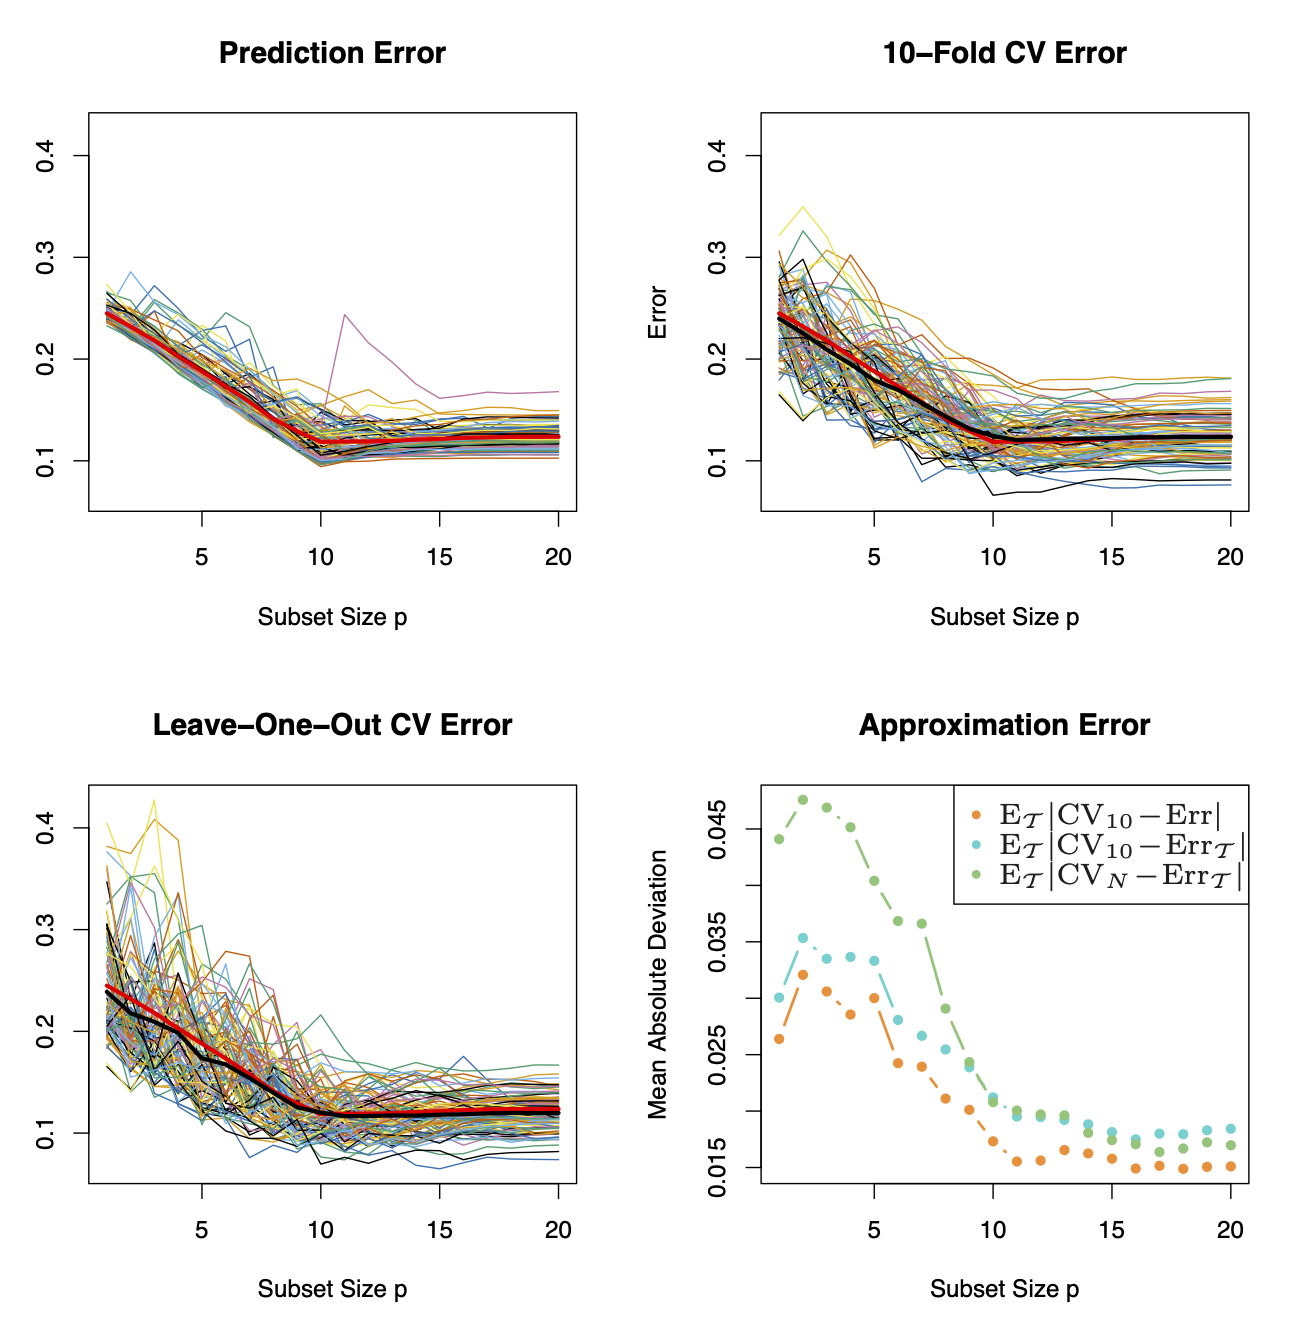
\includegraphics[width=0.8\textwidth]{figs/ESL_7_14.png}
\end{figure}

\end{frame}


% TODO: Add?

%\begin{frame}{LOO-CV for large data}

%\[
%CV(\hat{f},\alpha) = \frac{1}{N}\sum^N_{i=1} L(y_i,\hat{y}_{-\kappa(i)}(x_i,\alpha)
%\]

%Lets use sampling theory!\\[3mm]\pause

%Difference estimator

%Good approximations of the optimism.

%\end{frame}

\begin{frame}{The role of the data generating process}

\begin{itemize}
\item we assume that testset and train set are different observations from the same data generating process
\[
\mathbf{d} = \{(y_i, \mathbf{x}_i), i = 1, ..., n\} \,\sim P_{y,x}
\]
\item Things that can go wrong:
\begin{itemize}
\item temporal leak/concept drift
\item duplicated observations
\item non-randomized data
\end{itemize}
\pause
\item Example: Evaluating prediction models for Elections
% TODO: Add examples from the bachelor theses
\end{itemize}


\end{frame}

\begin{frame}<handout:0>{Questions?}
Questions?
\end{frame}

%%%%%%%%%%%%%%%%%%%%%%%%%%%%%%%%%%%%%%%%%%%%%%%%%%%%%%%%%%%%%%%%%%

\section{Regularisation}
\frame{\sectionpage}

\begin{frame}{Regression and GLM}
\begin{itemize}
\item Linear regression and logistic regression are examples of {\color{uured}generalised linear models}, GLMs.\\[3mm]\pause
\item Both use maximum likelihood estimation for fitting the model, where the likelihood function $L(\beta)$ is maximised.
\end{itemize}
\end{frame}

\begin{frame}{Regularised regression models}
\begin{itemize}
\item In some situations, for instance when the predictors are highly collinear, when there are too many predictors or when there is complete separation in the data, maximum likelihood estimation is unstable.\pause
\begin{itemize}
\item Either the solution is not unique, or minuscule changes in the data can change the solution completely.\pause
\item Such datasets are increasingly common in e.g. genomics, finance, astronomy and image analysis.\\[3mm]\pause
\end{itemize}

\item In such cases, {\color{uured}regularisation/shrinkage methods} can be used instead.\\[3mm]\pause
\item In a regularized GLM, it is not the likelihood $L(\beta)$ that is maximized, but a {\color{uured}regularised} function $L(\beta) \cdot p(\beta)$, where $p$ is a penalty function that typically forces the resulting estimates to be closer to 0, which leads to a stable solution.
\end{itemize}
\end{frame}

\begin{frame}{Regularised regression models}
Regularised linear regression models increase the {\color{uured}bias} of the estimates, but lowers their {\color{uured}variance}, thereby potentially decreasing the MSE.
\end{frame}

\begin{frame}{Connection to Bayesian estimation}
In Bayesian estimation, a {\color{uured}prior distribution} $p(\beta)$ for the parameters $\beta_i$ is chosen.\\[3mm]\pause
The estimates are then computed from the conditional distribution of the $\beta_i$ given the data, called the {\color{uured}posterior distribution}.\\[3mm]\pause
Using Bayes' theorem, we find that
$$P(\beta|\mathbf{x})\propto L(\beta)\cdot p(\beta),$$
i.e. that the posterior distribution is proportional to the likelihood times the prior.\\[3mm]
A special type of Bayesian estimator is the {\color{uured}maximum a posteriori (MAP)} estimator, which is found by maximizing the above expression (i.e. finding the mode of the posterior).\\[3mm]
This is equivalent to the estimates from a regularised frequentist model with penalty function $p(\beta)$!
\end{frame}

\begin{frame}{Inference and invariance}
\begin{itemize}
\item Regularised regression models are not invariant under linear rescaling of the predictors.\pause
\begin{itemize}
\item If a predictor is multiplied by a scalar $a\neq 0$, this can change the entire model.\pause
\item A model with measurements in inches might yield completely different results from a model with measurements in cm.\\[3mm]\pause
\end{itemize}
\item For this reason, it is widely agreed that the predictors should be standardized to have mean 0 and variance 1 before a regularised model is fitted.\pause
\begin{itemize}
\item With this approach we choose a particular (natural?) scaling, among all possible scalings.\pause
\item All predictors are on the same scale and are therefore treated equally by the penalty function.\pause
\end{itemize}
\end{itemize}
\end{frame}

\begin{frame}{Inference and invariance}
\begin{itemize}
\item Hypothesis tests are available (e.g. Lockhart et al. (2014), A significance test for the lasso, \emph{Annals of Statistics}), but I advise against using them.\\[3mm]\pause
\item Note that the hypothesis tests will be conditioned on the choice of scaling.\pause
\begin{itemize}
\item Because of this, regularised models are not appropriate for hypothesis testing -- the p-values could change completely if we rescaled the data!\\[3mm]\pause
\end{itemize}
\item Regularised regression models are however very useful for {\color{uured}predictive modelling}.
\end{itemize}
\end{frame}

\begin{frame}{$L_q$-penalties}
The most popular penalty terms correspond to common {\color{uured}$L_q$-norms}. \pause On a log-scale, the function to be maximized is
$$\ell(\beta)+\lambda\sum_{i=1}^p|\beta_i|^q,$$
where $\ell(\beta)$ is the loglikelihood of $\beta$ and $\sum_{i=1}^p|\beta_i|^q$ is the $L_q$-norm, with $q\geq 0$.\\[3mm]\pause
This is equivalent to maximizing $\ell(\beta)$ under the constraint that $\sum_{i=1}^p|\beta_i|^q\leq\frac{1}{h(\lambda)}$, for some increasing positive function $h$.\pause
\begin{itemize}
\item Relies on the {\color{uured}sparsity} assumption that most $\beta$ are 0.\\[3mm]\pause
\end{itemize}
$\lambda\geq 0$ is a {\color{uured}smoothing parameter}:
\begin{itemize}
\item When $\lambda=0$, we are back at the standard ML-estimate.
\item The $\hat{\beta}$ are forced to be closer to 0 when $\lambda$ increases.
\item $\lambda$ is usually chosen using cross-validation.
\end{itemize}
\end{frame}


\begin{frame}{Ridge regression}
When the $L_2$ penalty is used, the regularised model is called {\color{uured}ridge regression}, for which we maximize
$$\ell(\beta)+\lambda\sum_{i=1}^p\beta_i^2.$$
\begin{itemize}
\item Invented and reinvented by several authors, from the 1940's onwards.\\[3mm]\pause
\item In a linear model, the OLS estimate is $\hat{\beta}=(\mathbf{X}^T\mathbf{X})^{-1}\mathbf{X}^T\mathbf{y}$, whereas the ridge estimate is $\hat{\beta}=(\mathbf{X}^T\mathbf{X}+\lambda \mathbf{I})^{-1}\mathbf{X}^T\mathbf{y}$. The $\lambda \mathbf{I}$ is the 'ridge'.\\[3mm]\pause
\item The $\beta_i$ can become very small, but are never pushed all the way down to 0.\\[3mm]\pause
\item In a Bayesian context, this corresponds to putting a standard normal prior on the $\beta_i$.
\end{itemize}
\end{frame}

\begin{frame}{Lasso}
When the $L_1$ penalty is used, the regularised model is called the {\color{uured}lasso} (Least Absolute Shrinkage and Selection Operator), for which we maximize
$$\ell(\beta)+\lambda\sum_{i=1}^p|\beta_i|.$$
\begin{itemize}
\item Introduced by Robert Tibshirani in 1996.\\[3mm]\pause
\item As $\lambda$ increases, more and more $\beta_i$ become 0.\pause
\begin{itemize}
\item Simultaneously performs estimation and variable selection!\\[3mm]\pause
\end{itemize}
\item In a Bayesian context, this corresponds to putting a standard Laplace prior on the $\beta_i$.
\end{itemize}
\end{frame}

\begin{frame}{Examples in R}
Functions for regularised generalized linear models (linear, logistic, Poisson, multinomial, and more) are available e.g. in the \texttt{glmnet} package for R.\\[3mm]\pause
The syntax used is somewhat different from that for \texttt{glm} and \texttt{lm}.\\[3mm]
\end{frame}


\begin{frame}{Generalizations}
Regularised models have been a hot research topics in the last 20 years. Some additional important models are:\pause
\begin{itemize}
\item {\color{uured}Elastic net:} a compromise between ridge and lasso, in which $$\ell(\beta)+\lambda_1\sum_{i=1}^p|\beta_i|+\lambda_2\sum_{i=1}^p\beta_i^2$$ is maximized.\pause
\begin{itemize}
\item Introduced by Zou and Hastie in 2005.\pause
\item Is better than the lasso at handling correlated predictors.\pause
\item Has two smoothing parameters that we need to choose.\pause
\item Available in the \texttt{glmnet} package.\\[3mm]\pause
\end{itemize}
\item {\color{uured}Group lasso:} a version of the lasso in which variables can be grouped before fitting the model. The group lasso then selects groups of variables rather than individual variables.\pause
\begin{itemize}
\item Introduced by Yuan and Lin in 2006.\pause
\item Useful e.g. when we have dummies for categorical variables (in contrast, the lasso may choose to only include the dummies for some of the categories).
\end{itemize}
\end{itemize}
\end{frame}






\end{document}
